\documentclass[../thesis.tex]{subfiles}

\begin{document}

\chapter{Background subtraction}
\label{chap:bkg}

While Daya Bay's design ensures a very pure sample of antineutrino events, a small contamination of backgrounds (at the percent level) is unavoidable. These backgrounds can be subdivided into \emph{correlated} and \emph{uncorrelated} backgrounds. The uncorrelated backgrounds consist entirely of accidental coincidences between singles events, and the rate and spectrum can be easily estimated from that of the singles (see \autoref{sec:accratecalc}). On the other hand, the correlated backgrounds are so named because the prompt and delayed pulses are correlated in time and space, as they both originate from a single underlying process. The correlated background in Daya Bay consists of four distinct processes, and each one requires its own technique for determining the rate and energy spectrum.

In this chapter, we discuss the measurement of each of these backgrounds. Once they have been measured, their scaled prompt spectra can be subtracted from that of the IBD candidates, allowing the oscillation fit to proceed with a purer prompt spectrum, albeit one with an additional uncertainty stemming from the background measurements. We carry out our own prediction of the rates of the two dominant backgrounds: accidental coincidences and $^9$Li/$^8$He decays. For the three other backgrounds (fast neutrons, AmC events, and $\CanO$), we use the results of the detailed studies that were carried out by members of the collaboration. Those background studies were considerably complex and carefully validated analyses in their own right, and we make no attempt to improve upon them.

Before considering these double-coincidence backgrounds, we begin by discussing a background defined at the level of \emph{individual} triggers, namely, the so-called ``flashing'' of PMTs. Reduction of these ``flashers'' is necessary in order to minimize the rate of the uncorrelated backgrounds. This reduction occurs at an early stage in the analysis (the ``pre-selection'', as described in \autoref{sec:selPreSel}), eliminating flashers entirely from further consideration.


\section{PMT light emission (``flashers'')}
\label{sec:bkgFlashersOverview}

The PMTs used at Daya Bay have the tendency to occasionally ``flash'', emitting light due to arcing in their bases. The rate and intensity of this ``flashing'' would change over time for each PMT. At any given moment, some 5\% of the PMTs in each AD will have the tendency to flash brightly enough to trigger the detector \cite{SideBySide}, in some cases producing as much as 100~MeV of reconstructed energy. Within the delayed energy region of 6-12~MeV, the flasher rate has averaged at around 0.7~Hz for each AD. These ``delayed-like'' flashers, if included in the analysis, would significantly increase the rate of backgrounds caused by the accidental coincidence of two uncorrelated signals. As discussed in \autoref{sec:accbkg} and \autoref{chap:accDMC}, the rate of such ``accidentals'' is proportional to the rate of delayed-like signals, and this rate (excluding flashers) ranges from around 0.05~Hz at EH3 to 1~Hz at EH1. While the flashers would merely (roughly) double the 1\% accidental background in the near halls, in the far hall they would increase this background by an order of magnitude to the 10\% level, counter to Daya Bay's goal of perecent-level background contamination.

\begin{figure}[h!]
  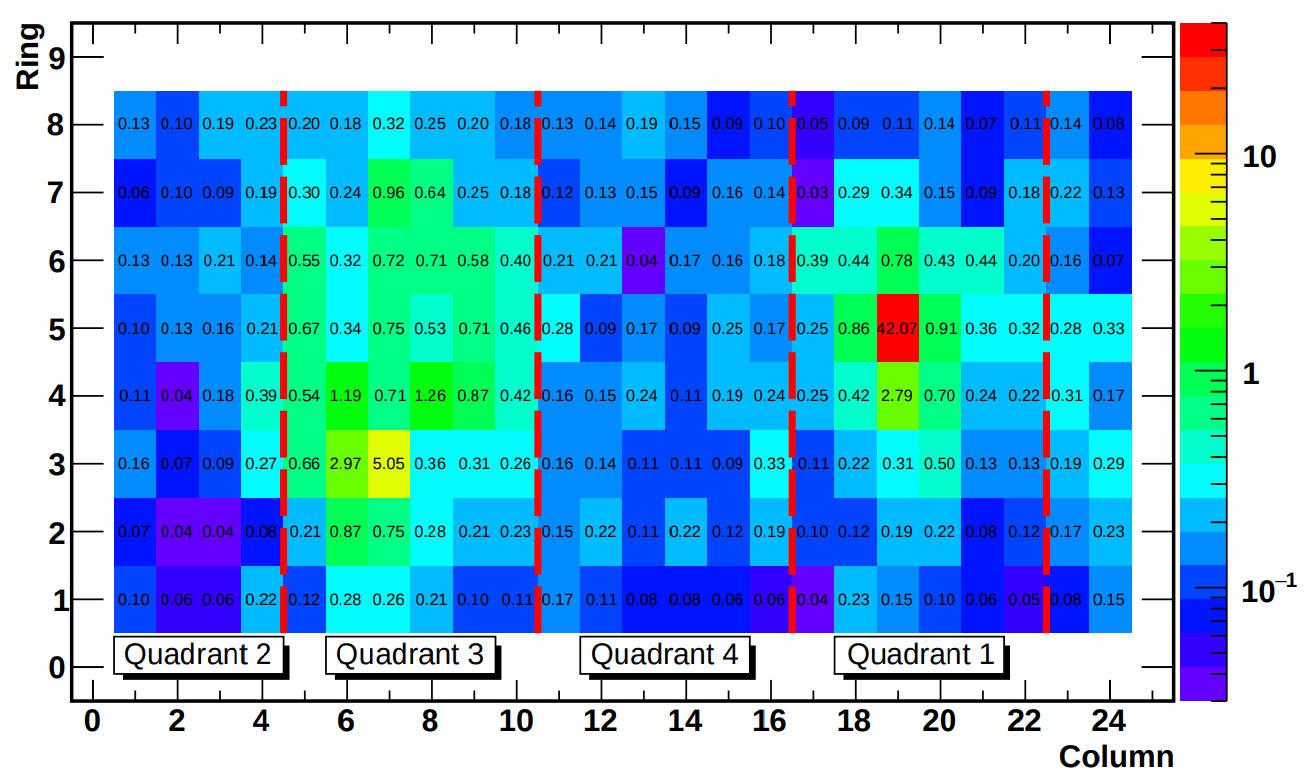
\includegraphics[width=\textwidth]{Backgrounds/Flasher/example_event.png}
  \caption{PMT charge distribution of a flasher candidate, illustrating the division of the AD into four azimuthal quadrants, with Quadrant 1 being centered around the PMT with the highest charge. From \cite{An_2017}.}
  \label{fig:flasher_exampleOverview}
\end{figure}

Fortunately, flashers are easily distinguished from ``physical'' singles due to their unique conical pattern of light emission (\autoref{fig:flasher_exampleOverview}), enabling them to be removed from the analysis with high efficiency while minimally affecting true IBDs. This light pattern is characterized by two ``hot spots'' on opposite sides of the AD. As described in \autoref{sec:bkgFlashers}, a highly effective discriminator can be used to reject flashers based on their charge and time patterns, respectively. This discriminator, denoted by $\fID$, is based on two variables. The first, $\fmax$, is the ratio of $Q_{\mathrm{max}}$ (the maximum individual PMT charge across all PMTs) over the total charge $Q_{\mathrm{tot}}$:
\begin{equation}
  \fmax = \frac{Q_{\mathrm{max}}}{Q_{\mathrm{tot}}}.
\end{equation}
The second, $\fquad$, is based on dividing the AD into four quadrants (\autoref{fig:flasher_example}): ``Quadrant 1'' (q1) is the one that is centered on the highest-charge PMT, q3 is the one across from q1, and q2 and q4 are the two ``to the side.'' Then, $\fquad$ captures the conical nature of the light emission:
\begin{equation}
  \fquad = \frac{Q_{\mathrm{q3}}}{Q_{\mathrm{q2}} + Q_{\mathrm{q4}}}.
\end{equation}
Individually, $\fmax$ and $\fquad$ do not cleanly distinguish flashers from physical events. Their combination, however, does, leading to the definition of $\fID$:
\begin{equation}
  \fID = \log_{10} \left[ \fquad^2 + \left( \frac{\fmax}{0.45} \right)^2 \right].
\end{equation}
Flashers can then be identified as those events having $\fID > 0$. As shown in \autoref{fig:bkgFlasherEllipse2DOverview}, this discriminator effectively eliminates flashers from the analysis. Complete elimination is unnecessary; all that matters is that the residual flashers do not significantly increase the rate of delayed-like singles (and hence accidentals). This is easily the case for the $\fID$ discriminator.

Although $\fID$ alone provides sufficient flasher rejection, even further rejection can be achieved by taking advantage of the characteristic time distribution of flashers. Since flashers involve the propagation of light between opposite walls of the AD, the time distribution is broadened in comparison to typical physical events. As such, we can use the discriminator
\begin{equation}
  \fPSD = \log_{10} [4 \cdot (1 - f_{\mathrm{t}1})^2 + 1.8 \cdot (1 - f_{\mathrm{t}2})^2]
\end{equation}
to identify flashers. Here, $f_{\mathrm{t}1}$ ($f_{\mathrm{t}2}$) is defined as the ratio of the number of hits in the first 200 (150)~ns of the signal, over the number of hits in the first 400~ns.

Finally, a third discriminator can be used to reject flashers from the 2" calibration PMTs located at the top and bottom of the AD. These events are identified as those in which any 2" PMT records more than 100 photoelectrons. Together, these three methods all but eliminate flashers from the data.

The exact rejection factor for flashers is unimportant, as long as it is high enough to avoid a significant rate of flasher-associated accidentals. Any residual flashers will automatically be counted in the singles rate, and thus so will their contribution to the accidental background rate. However, it \emph{is} important to study the \emph{signal inefficiency} of the flasher rejection, that is, the proportion of non-flashers that incorrectly get identified as flashers. As discussed in \autoref{sec:bkgFlasherEffs}, this inefficiency has been found to be $0.039\% \pm 0.006\%$, with no significant AD-to-AD variation. This 0.006\% uncertainty is rounded up to 0.01\% and included in the detection efficiency uncertainty (\autoref{tab:detEff}).

\begin{figure}[ht!]
  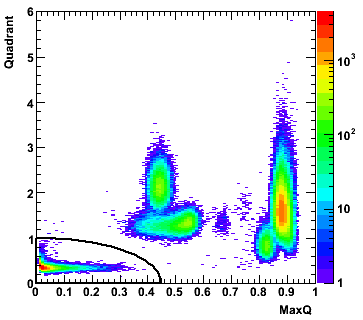
\includegraphics[width=0.5\textwidth]{Backgrounds/Flasher/ellipse_2d.png}
  \caption{Two-dimensional distribution of $\fmax$ (``MaxQ'') and $\fquad$ (``Quadrant'') for physical triggers in EH1-AD2. The black ``ellipse'' corresponds to $\fID = 0$; events outside the ellipse are identified as flashers. High flasher rejection and negligible signal inefficiency are apparent. From \cite{flasherControl}.}
  \label{fig:bkgFlasherEllipse2DOverview}
\end{figure}

\section{Accidental coincidences}
\label{sec:accbkg}

IBD-like pairs can be formed when two uncorrelated triggers (\emph{singles}) ``accidentally'' occur closely together in time. Given that the prompt-like singles rate (after flasher rejection) is approximately 50~Hz in each AD,\footnote{Meanwhile, the delayed-like singles rate ranges from $\sim$0.001~Hz at the far site to $\sim$0.1~Hz at the near sites; this is still large enough to provide ample statistics from Daya Bay's multi-year dataset.} the characteristics of singles (and thus of accidentals) can be measured with extremely high statistical precision. Once the rates of prompt-like and delayed-like singles have been determined, the accidentals rate can be calculated via a straightforward application of Poisson statistics. This procedure is detailed in \autoref{sec:accratecalc}. The spectrum, meanwhile, is equal to that of the singles sample, whose extraction is described in \autoref{sec:selSingles}. In \autoref{sec:accStatUnc} and \autoref{sec:accSystUnc} we discuss the statistical and systematic uncertainty on the accidentals rate; in total, a conservative uncertainty of 2\% is assigned to the rate for all ADs and data periods.

\begin{comment}
As previously stated, the accidental background can be straightforwardly measured based on the characteristics of singles events. The singles spectrum is first measured by searching for prompt-like events that satisfy the usual muon vetos but are separated from other prompt-like events by at least 400~$\mu$s. The total integral of this spectrum gives the prompt-like rate $R_p$, while the integral above 6~MeV gives the delayed-like rate $R_d$. The accidental background rate is then simply
\[ R_\mathrm{acc} = R_d(1 - e^{-R_p\Delta t})e^{-2R_p\Delta t}, \] where the factor in parentheses is the probability for a prompt-like single to fall within the $\Delta t$~=~200~$\mu$s preceding a delayed-like single, and the final factor is the probability that the event is \emph{not} rejected by the decoupled multiplicity cut, which disallows any additional prompt-like single in the 400~$\mu$s preceding the delayed event. Once the rate has been determined this way, the spectrum is trivial: It is simply the singles spectrum itself.
\end{comment}

\begin{comment}
  Mention IHEP's cross-check, and the additional uncertainty stemming from the difference between it and the nominal result?
\end{comment}

\section{Cosmogenic $^9$Li/$^8$He}
\label{sec:bkgCosmo}

\newcommand\linine{$^9$Li}

The dominant correlated background for Daya Bay comes from the isotopes $^9$Li and $^8$He, which are produced as spallation products of carbon when energetic muons traverse the AD. These two isotopes have relatively long lifetimes of 257~ms for $^9$Li and 172~ms for $^8$He \cite{ENDF} (see \autoref{tab:bkgLi9He8Props}); thus, while the majority of them will decay within the O(1~s) veto window that follows showering muons, a non-negligible fraction will survive past it. As shown in \autoref{fig:li9he8_decays}, when one of these isotopes undergoes beta decay into the relevant excited states of the daughter nucleus, the daughter will immediately emit a neutron (and, in the case of $^9$Li, will further disintegrate into two alpha particles). The relevant $\beta$ decay endpoints extend up to 12~MeV, placing these decays squarely within the IBD prompt-energy region. The combination of this $\beta$ decay and the subsequent nGd capture produces the characteristic double-coincidence signature of an IBD event. In what follows, we will collectively refer to these two isotopes as $^9$Li, given that it is believed to be the predominant of the two. (For instance, the KamLAND collaboration's FLUKA simulations \cite{KamLAND_cosmo} indicated a 10:1 ratio of $^9$Li to $^8$He production.\label{par:kamland_he8}\footnote{Given KamLAND's higher $\langle E_\mu \rangle$ of 260~GeV, compared to Daya Bay's $\sim$50 (100) GeV at the near (far) site(s), KamLAND's measured ratio of $^9$Li to $^8$He may not be completely representative, but in the absence of additional data, it is an acceptable starting point. In practice, as discussed later, we use a nominal (and somewhat arbitrary) $^8$He fraction of 5.5\%, with other values trialed as part of the overall uncertainty estimation.}) Later we will propagate the uncertainty on this ratio into the background estimation. 

\begin{table}[h]
  \begin{tabular}{lccc}
    \toprule
    Isotope & Lifetime (ms) & $\beta$ decay endpoint (MeV) & Final products \\
    \midrule
    $^9$Li & 257.2 & 11.17 & $e^-$ + $\alpha$ + $\alpha$ + n (+ $\nuebar$)\\
    $^8$He & 171.6 & 7.44 & $e^-$ + $^7$Li  + $\gamma$ + n (+ $\nuebar$)\\
    \bottomrule
  \end{tabular}
  \caption{Properties of the cosmogenic isotopes $^9$Li and $^8$He \cite{ENDF}. The quoted $\beta$ decay endpoint is the endpoint of the highest-energy transition \emph{that produces a final neutron}.}
  \label{tab:bkgLi9He8Props}
\end{table}

\begin{figure}[h]
  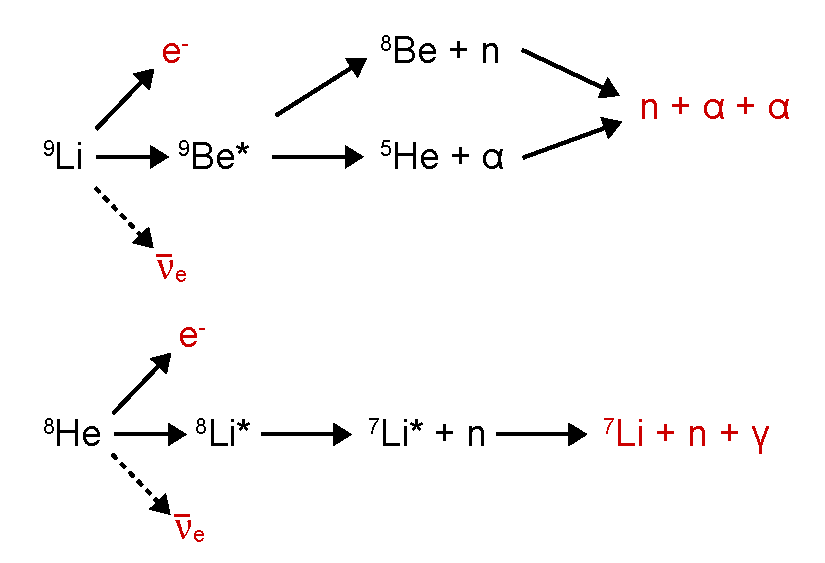
\includegraphics[scale=0.75]{Backgrounds/li9he8_decays.pdf}
  \caption{Decay cascades of $^9$Li and $^8$He with excited daughter nuclei after $\beta$ decays. Final products are highlighted in red. Extended from \cite{pedroLi9Spec2}.}
  \label{fig:li9he8_decays}
\end{figure}

Although at Daya Bay there is no feasible way of distinguishing \linine\ decays from IBDs at the level of individual events, it is still possible to statistically estimate the total \linine\ rate by exploiting the correlation in time between \linine\ events and preceding muons. To see this, let the muon rate be denoted by $R_\mu$, and the \linine\ livetime by $\tau$. Since IBD events are uncorrelated with muons, the time between an IBD and the most recent preceding muon is given, according to Poisson statistics, by the probability density function (PDF)
\begin{equation}
  \label{eq:cosmoBkgPdfIbd}
  f_{\mathrm{IBD}}(t) = R_\mu e^{-R_\mu t}.
\end{equation}
Meanwhile, a \linine\ decay is correlated in time with the parent muon:
\begin{equation}
  \label{eq:cosmoBkgPdfLiProd}
  f_{\mathrm{Li,\,Parent}}(t) = \frac{1}{\tau} e^{-t/\tau}.
\end{equation}
However, in the time between a muon shower and an associated \linine\ decay, additional muons may be detected, and these may closely resemble the true parent muon. As such, the quantity that we can reliably measure is not the time between the \linine\ decay and the parent muon, but (as with IBDs) the time between the decay and the \emph{last} muon. This detail has the effect of modifying the time constant in \autoref{eq:cosmoBkgPdfLiProd}. To derive this modification, let us consider a \linine\ event with a time-to-last-muon of $t$. Either the last muon was the parent muon, or it wasn't. Defining our time axis with the decay at the origin, these two possibilities can be stated quantitatively as:
\begin{enumerate}
\item The parent muon occured at time $-t$, with no intervening uncorrelated muons, or
\item The parent muon occured at some (unknown) time prior to $-t$, and the most recent uncorrelated muon occured at $-t$.
\end{enumerate}
The parent muon's time PDF is given by \autoref{eq:cosmoBkgPdfLiProd}, and that of the most recent uncorrelated muon by \autoref{eq:cosmoBkgPdfIbd}. Meanwhile, the Poisson probability of observing zero uncorrelated muons in a time window of $t$ is given by $e^{-R_\mu t}$. Thus, letting $P_1$ and $P_2$ be the probabilities\footnote{Here we will say ``probability'' when we really mean ``probability density''.} of the two cases above, we have
\begin{align*}
  P_1 = \frac{1}{\tau} e^{-t/\tau} \cdot e^{-R_\mu t} = \frac{1}{\tau}e^{-(R_\mu + 1/\tau)t}
\end{align*}
and
\begin{align*}
  P_2 = \int_t^\infty \frac{1}{\tau}e^{-t'/\tau}\,dt' \cdot R_\mu e^{-R_\mu t} = e^{-t/\tau} \cdot R_\mu e^{-R_\mu t} = R_\mu e^{-(R_\mu + 1/\tau)t}.
\end{align*}
Letting
\begin{equation}
  \lambda = R_\mu + 1/\tau,
\end{equation}
we finally add $P_1$ and $P_2$ to obtain the PDF of time-to-last-muon for \linine\ decays:
\begin{equation}
  \label{eq:cosmoBkgPdfLi}
  f_{\mathrm{Li}}(t) = \lambda e^{-\lambda t}.
\end{equation}

Comparing \autoref{eq:cosmoBkgPdfLi} and \autoref{eq:cosmoBkgPdfIbd}, we see that, if $\lambda$ is sufficiently different from $R_\mu$ (in other words, if $R_\mu$ is sufficiently small relative to $1/\tau$), then there will be a measurable difference between the time-to-last-muon PDFs of \linine\ and IBD events. In this case, the separate event counts can be obtained by constructing a histogram of time-to-last-muon from a mixed sample of IBDs and \linine\ events. This histogram can then be fit to a weighted sum of \autoref{eq:cosmoBkgPdfLi} and \autoref{eq:cosmoBkgPdfIbd}, with the weights (as detemined by the fit) corresponding to the number of events in the two categories:
\begin{equation}
  f(t) = N_{\mathrm{Bkg}} \lambda e^{-\lambda t} + N_{\mathrm{IBD}} R_\mu e^{-R_\mu t}.
\end{equation}

If the fit is allowed to extend down to $t$ of a couple dozen ms, an additional correlated component must be considered resulting from accidental double coincidences of $^{12}$B and/or $^{12}$N decays. These two isotopes, with respective lifetimes of 29 and 16~ms \cite{ENDF}, and $\beta^\pm$ endpoints of 13.7 and 16.3~MeV \cite{ENDF}, can be produced multiple times by a single muon shower, and their decays extend well into the delayed-energy region. Their double coincidences are already considered as part of the accidental background estimation\footnote{There is some bias owing to the fact that the prompt and delayed $^{12}$B/$^{12}$N are not uncorrelated in time (as assumed in the accidentals calculation), but are in fact correlated by virtue of their usually coming from the same parent muon. However, the rate of such events is extremely low (relative to the total accidentals rate), as can be seen in the fits shown later in this chapter, so there is no need to attempt a correction to the accidentals rate.}, so we are not concerned with measuring them here as a separate background; however, they do distort the time-to-last-muon histogram at low times, and thus they must be considered in order to extract the \linine\ component accurately. Past fits \cite{NonlinearityPaper} to the spectrum of muon-correlated singles have indicated that $^{12}$B is by far the dominant of these isotopes (comprising some 97\% of the events), so in what follows we treat it as the only one of relevance.

When fitting the time-to-last-muon for the $^{12}$B double coincidences (BB events, for short), the time constant must be considered carefully. We first consider the time to the \emph{parent} muon, rather than to the \emph{last} muon. For the single $^{12}$B events, the corresponding time constant is simply the $^{12}$B lifetime $\tau_{\mathrm{B}}$.  However, if a muon produces two $^{12}$B nuclei, then a timespan of $t$ will correspond to an $e^{-t/\tau_{\mathrm{B}}}$ survival probability of one nucleus, and likewise for the other. The observation of one decay, of either nucleus, constitutues an observation of the whole pair, since we are recording the time between muons and the \emph{prompt} event in an IBD candidate. The probability of not observing the pair, then, is the probability of seeing \emph{neither} nucleus decay, which is $(e^{-t/\tau_{\mathrm{B}}})^2 = e^{-t/(\tau_{\mathrm{B}}/2)}$. That is, the time constant for the BB time-to-parent-muon distribution is $\tau_{\mathrm{B}}/2$. For the time to the \emph{last} muon, rather than the parent, the arguments preceding \autoref{eq:cosmoBkgPdfLi} then imply a rate constant of $\lambda_{\mathrm{BB}} = R_\mu + 2/\tau_{\mathrm{B}}$.
\begin{comment}
\footnote{We neglect the possibility of only seeing \emph{one} of the nuclei decay, since the IBD coincidence cut of \us{200} is far shorter than the $^{12}$B lifetime of 29~ms, and therefore, the observation of one decay effectively \emph{implies} the observation of the other.}

 As such, the time constant for BB events is $\tau_{\mathrm{B}}/2$. (I'm not sure I buy this. We are \emph{assuming} that the two decays occur within 200~us of each other, and the probability of seeing them both is basically equivalent to the probability of seeing the first, and the time-to-last-muon PDF for the first just has the time constant of $\tau$. Where the time constant \emph{does} get halved is if we consider a muon that produces two nuclei and we want the probability of seeing none i.e. the time to the next decay.)
\end{comment}

\begin{comment}
  YYY our code has the 12B half-life (20 ms) listed as the lifetime (should be 29 ms). This further exacerbates the use of the mistaken(???) factor of 2??? In total our time constant has been off by a factor of 3 (well, plus the Rmu part)
\end{comment}

To finish deriving the full expression used in fitting the time to last muon, we simply add a factor $r$ corresponding to the $^8$He fraction, giving
\begin{equation}
  \label{eq:bkgLi9FullExpr}
  f(t) = N_{\mathrm{Bkg}} \left[ (1-r)\lambda_{\mathrm{Li}} e^{-\lambda_{\mathrm{Li}} t} + r\lambda_{\mathrm{He}} e^{-\lambda_{\mathrm{He}} t }\right] + N_{\mathrm{BB}} \lambda_{\mathrm{BB}} e^{-\lambda_{\mathrm{BB}} t} + N_{\mathrm{IBD}} R_\mu e^{-R_\mu t},
\end{equation}
where
\begin{align*}
  \lambda_{\mathrm{Li}} &= R_\mu + 1/\tau_{\mathrm{Li}} \\
  \lambda_{\mathrm{He}} &= R_\mu + 1/\tau_{\mathrm{He}} \\
  \lambda_{\mathrm{BB}} &= R_\mu + 2/\tau_{\mathrm{B}}.
\end{align*}

Although this method is simple in theory, a significant challenge arises from the fact that a minimum muon energy must be defined when calculating the time between each event and its most recent preceding muon. If this cut is too low, then the time between muons will be comparable to (or smaller than) the \linine\ livetime, and with finite statistics, it will be difficult to reliably distringuish between the two components in the fit. Conversely, if the muon cut is too high, then some fraction of \linine-producing muons will be discarded, and those \linine\ events will not appear to be muon-correlated, leading to an underestimation of the rate.

This issue is mitigated somewhat by the fact that low-energy muons produce a relatively small portion of the total \linine\ rate.\footnote{More precisely, at the near (far) sites, some 80\% (90\%) of the $^9$Li in the IBD sample comes from muons of visible energy above 1~GeV. This can be deduced from the results shown in \autoref{tab:bkgLi9Rates} (where 1~GeV $\sim$ 160,000 photoelectrons).}
% Note: See /home/mkramer/apps/spacemacs/.emacs.d/.cache/junk/2020/11/28-li9frac.jl
However, an accurate assessment must still attempt to quantify the contribution from low-energy muon events. To enhance the \linine\ signal in the fit, either the muon sample or the \linine\ candidate sample (or both) must be somewhat purified. Purifying the muon sample will enhance the difference in time constants between the $^9$Li and IBD components, while purifying the $^9$Li sample will enhance the difference in amplitudes. We use both methods in what follows.

For the muon sample, the goal is to remove muons that are unlikely to produce a \linine\ event. This will reduce the muon rate $R_\mu$, thus increasing the difference between the time constants of the fit components. However, the cost of this \emph{muon reduction} is that some fraction of \linine-producing muons will be discarded. The associated \linine\ events will have a time-to-last-muon rate constant of $R_\mu$ rather than $\lambda$, so they will not contribute to the measured \linine\ rate, leading to an inefficiency (and corresponding uncertainty) in the total rate estimate. Here, muon reduction is achieved by using \emph{neutron tagging}, in which we only consider those muons for which a neutron capture candidate is observed in the immediate aftermath. Given the sizable uncertainty on the efficiency of the tagging, this method is only used where absolutely necessary, i.e., in the bin of the lowest muon energy. The details are discussed later.

As for increasing the purity of the \linine\ sample, the method used here is simply to apply a cut on the prompt energy. As can be seen by comparing \autoref{fig:li9_spec} to \autoref{fig:selPromptSpec}, the \linine\ and IBD spectra differ substantially, with the former being much harder. As such, a higher prompt-energy cut will increase the ratio of \linine\ to IBD events. This benefit, however, must be weighed against the loss in the total statistics arising from an aggressive prompt-energy cut. Here, heuristically chosen cuts are used in order to obtain acceptable fits. As will be detailed later, more aggressive cuts are used in the near hall (where the IBD ``background'' fraction is larger) and for lower muon energies (where a greater \linine\ purity is needed due to the proximity of $\lambda$ to $R_\mu$). These prompt cuts, together with neutron tagging (for low muon energies), enable the \linine\ fit to be performed for muon energies that extend all the way down to the ``AD muon'' threshold of 3,000~pe.

In the sections that follow, we describe the \linine\ rate estimation in detail, beginning with the selection of \linine\ candidates, followed by the muon selection, the fitting procedure, its results, the various selection efficiencies, and the error budget. Our method is a repeated and slightly modified version of the one described by Chris Marshall in \cite{ChrisLi9}, which in turn was based on a 2014 analysis performed by the author in \cite{MattLi9}.

\subsection{$^9$Li candidate selection}
\label{sec:bkgLi9Sel}

The $^9$Li selection is largely identical to the standard IBD selection, as described in \autoref{chap:selection}, but with two key differences: First, the prompt-energy cut is higher, as described above (although this cut is applied after the initial selection, for the sake of flexibility), and, secondly, the ``shower muon'' veto is disabled. That is, rather than vetoing for 0.4004~s after a muon of $>$300,000~pe (as in our nominal IBD selection), only the ``AD muon'' veto of 1.4~ms is applied. This is necessary because the shower veto would otherwise remove a large fraction of the $^9$Li events, greatly reducing the already-limited statistics of the sample. More precisely, for a given $^9$Li event produced by a shower muon, the probability of its falling within the veto window is
\begin{equation}
  \label{eq:bkgLi9VetoProb}
  1 - \exp\left( - \frac{400.4}{257} \right) \approx 80\%,
\end{equation}
where the numerator is the veto time and the denominator is the $^9$Li lifetime (in milliseconds, in both cases). As shown in \autoref{tab:bkgLi9Rates}, some 90\% of $^9$Li events are produced by shower muons. Multiplying this percentage by that from \autoref{eq:bkgLi9VetoProb} implies that some 70\% of $^9$Li events would be lost if the shower veto were applied. A similar argument applies for $^8$He.

When producing the final \linine\ rate estimation, we must correct for the efficiency of this modified muon veto. Using the muon toy MC described in \autoref{sec:cutVaryMuVetoEff}, these efficiencies were determined to be 87\%, 90\%, and 99\% in EH1, EH2, and EH3, respectively. (Compare to 82\%, 85\%, and 98\% for the standard muon veto.)

% YYY the Li9 rates, as I've been using them so far, are calculated assuming the efficiencies of the standard muon veto, rather than the modified one. I've corrected the constants in Li9Calc accordingly, but need to rerun the calculation and update the plots etc. ... I think I fixed it in yolo4 and oct20v3?

\subsection{Muon selection}
\label{sec:bkgLi9MuonSel}

For the purposes of applying the muon veto and constructing the time-to-last-muon distributions, we use the muon tree generated by the Daya Bay software framework (\texttt{NuWa}) during data production, as discussed in \autoref{sec:selProd}. In this tree, muons that trigger multiple detectors are merged into a single muon, and prompt retriggers are discarded. This represents a minor difference from our IBD selection, where retriggers are \emph{not} discarded, leading to a slight reduction in our muon veto efficiency compared to what we'd obtain from using the \texttt{NuWa} muon tree. (This difference is correctly accounted for in the summation of veto windows, and thus there is no resulting bias.) For the $^9$Li analysis, the removal of retriggers helps to prevent any biasing of the time constant for $^9$Li events. The \texttt{NuWa} muon selection's cuts are designed to be looser than any conceivable muon definition used in a physics analysis (which would in turn select a subset of \texttt{NuWa's} ``muons''). Accordingly, they are as follows:

\begin{itemize}
\item A trigger in the inner (outer) water pool, with at least 6 (8) fired PMTs, is tagged as a WP muon.
\item A trigger in an AD of more than 3000 photoelectrons is tagged as an AD muon.
\item Tagged muons that occur within a 300~ns window are merged into a single muon (with the WP hit counts and AD charges individually stored), with the timestamp taken to be the time of the earliest trigger.
\item Any subsequent ``muons'' that occur within 10~\us\ are deemed to be retriggers and are thus discarded.
\end{itemize}

During the $^9$Li selection, a given muon object will result in the 1.4~ms AD muon veto if the object contains an AD muon for the detector in question. If not, but if there is a IWP or OWP muon present with \emph{more than 12 hit PMTs}, then the 600-\us\ WP muon veto is applied instead.

If a $^9$Li candidate is found, then all preceding muons within a 10-second window are stored in an array specific to that candidate. This array can then be looped over when constructing the time-to-last-muon histogram, skipping over muons outside of a chosen energy range until the most recent one within the energy range is found.

\subsubsection{Neutron tagging}
\label{sec:bkgLi9NeuTag}

In order to enable the neutron tagging technique (as needed for calculating the rate of $^9$Li produced by low-energy muons), an additional flag is stored for each muon, indicating whether the muon occurred in coincidence with a neutron capture candidate. Specifically, the neutron tag is applied if any trigger ranging from 1.8 to 12~MeV
% (YYY why is it 18~MeV in the code?)
occurs between 20 and 200~\us\ after the muon. Although these cuts are heuristic, they are reasonable in principle: The energy range is wide enough to include captures on both gadolinium and hydrogen, and the time window includes most of the Gd captures and a decent fraction of H captures, while avoiding spurious signals that can arise from retriggers occurring in the first dozen or so \us\ after a muon.

The primary challenge in using the neutron tagging technique is accounting for the efficiency of the tagging. That is, what percentage of $^9$Li-producing AD muons (within a specified energy range) will be neutron-tagged? For sufficiently high-energy muons (roughly above 160,000 photoelectrons), the $^9$Li rate can be measured both with and without neutron tagging, and thus the efficiency can be extracted directly. However, for muons below 160,000~pe (where neutron tagging is unavoidable), this is not possible, and the efficiency must be extrapolated. We discuss this efficiency, and its uncertainty, in \autoref{sec:bkgLi9NeuTagEff}.
% In \cite{WeiLi9}, the efficiency is measured across a range of muon energies, and found to range from $\sim$90\% for muons above 1.8~GeV ($\sim$290,000~p.e.), down to $\sim$60\% for muons of 1.0--2.5~GeV (1.6--4e5~p.e.). For the sake of analysis, we thus assume a neutron tagging efficiency of 60\% (YYY need to fix this in Li9Calc and generate new results!!!), and apply a corresponding relative uncertainty of 45\% to the $^9$Li rate for muons below 160,000~p.e.

\subsection{Time-to-last-muon fit}
\label{sec:bkgLi9HistoFit}

Once a sample of $^9$Li candidates has been collected, along with the history of prior muons for each such candidate, the next step is to construct the histogram of times since the most recent muon (within a given muon energy range). We use a histogram spanning from 2~ms to 1~s, with a nominal binning consisting of 24 variable-width bins. The lowest bin covers 2 to 20~ms; the next four bins (up to 100~ms) are 20-ms-wide; the next four (up to 0.5~s) are 0.1-s-wide; the next six (up to 2~s) are 0.25-s-wide; the next two (up to 3~s) are 0.5-s-wide; and the final seven are 1-s-wide. This variable binning scheme captures the fine structure at low times while keeping the number of bins at a manageable level. Later we discuss the systematic uncertainty arising from variation of the binning.

For each hall, three histograms were constructed, corresponding to three muon visible energy ranges of $<$160,000, 160,000-300,000, and $>$300,000~pe.\footnote{As detailed in \autoref{chap:cutVary}, we later vary the definitions of these ranges in order to capture the dependence of the final $^9$Li rate on the muon energy used in the definition of the shower muon veto. The ranges described here apply to the shower veto used in the nominal IBD selection.} Different cuts are used in the three ranges, as detailed in \autoref{tab:bkgLi9Cuts}. To fill each histogram, we loop over all $^9$Li candidates for the hall in question, and if the candidate is accepted by the prompt-energy cut, we then find the most recent preceding muon (within the specified energy range, and with a neutron tag when required). The time between the candidate and the muon is then used to fill the histogram.

\begin{table}[h]
  \centering
  \begin{tabular}{lccc}
    \toprule
    Hall & PE range ($\times10^3$) & Prompt cut (MeV) & Neutron tag? \\
    \midrule
    EH1/2  & 5-160   & 8.0 & Yes \\
           & 160-300 & 8.0 & No  \\
           & 300-inf & 3.5 & No  \\
    \midrule
    EH3  & 5-160   & 6.0 & Yes \\
         & 160-300 & 6.0 & No  \\
         & 300-inf & 3.5 & No  \\
    \bottomrule
  \end{tabular}
  \caption{Cuts used in constructing the three separate time-to-last-muon histograms for each hall.}
  \label{tab:bkgLi9Cuts}
\end{table}

After constructing the histogram, we fit it to \autoref{eq:bkgLi9FullExpr}. The results are shown in Figures~\ref{fig:li9_fits_eh1}--\ref{fig:li9_fits_eh3}. For the nominal result, we fix the $^8$He fraction $r$ to be 5.5\% (an inherited ``reasonable guess'', as discussed further in \autoref{sec:bkgLi9Spectrum}), and include the $^{12}$B component. Later we discuss the effects of varying the $^8$He fraction and the inclusion of $^{12}$B. The best-fit value of $N_{\mathrm{Bkg}}$, as determined by \texttt{MINUIT}, corresponds to the raw number of (muon-correlated) $^9$Li/$^8$He events present in the sample used for filling the histogram. As discussed in \cite{ChrisLi9}, the fit does not suffer from any appreciable correlation between $N_{\mathrm{Bkg}}$ and $N_{\mathrm{IBD}}$, as the latter is strongly constrained by the tail at high time-to-last-muon. This was verified in \cite{ChrisLi9} by hand-scanning the variation of $\chi^2$ as a function of $N_{\mathrm{Bkg}}$. Thus, \texttt{MINUIT's} reported statistical uncertainty on $N_{\mathrm{Bkg}}$ can be safely taken at face value and propagated into our final uncertainty. Our fit results are summarized in \autoref{tab:bkgLi9Rates}. As discussed further in \autoref{chap:cutVary}, the fit was also performed using alternative muon energy ranges, in order to characterize the dependence of the $^9$Li rate on the choice of shower-muon threshold.

\begin{figure}[ht]
  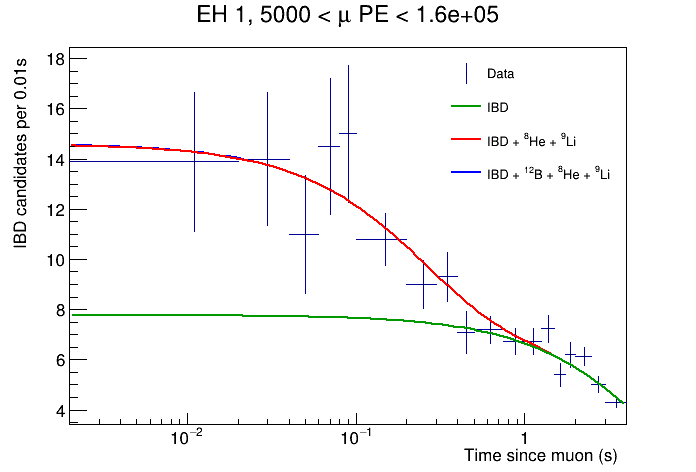
\includegraphics[width=0.5\linewidth]{Backgrounds/Li9/fits/EH1_range1_CV_logx.png} \\[0.5em]
  \begin{minipage}{0.5\textwidth}%
    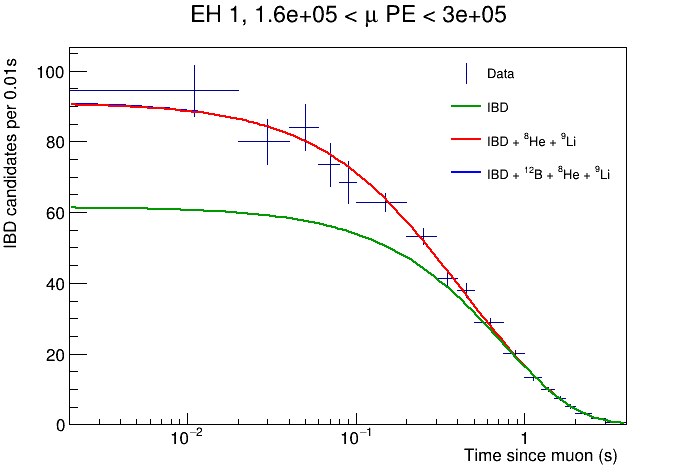
\includegraphics[width=\linewidth]{Backgrounds/Li9/fits/EH1_range2_CV_logx.png}%
  \end{minipage}%
  \begin{minipage}{0.5\textwidth}%
    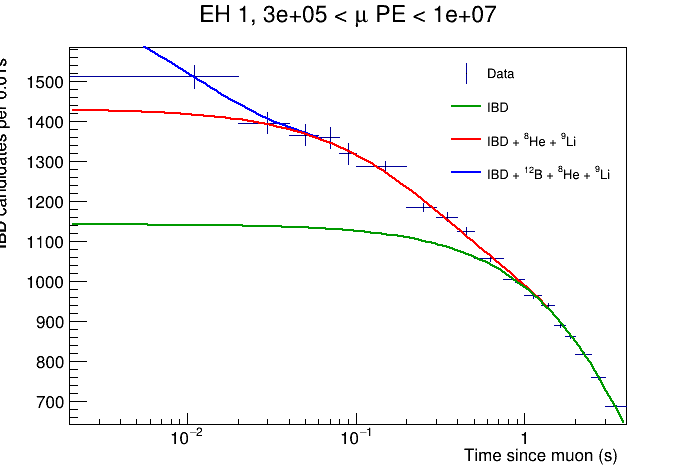
\includegraphics[width=\linewidth]{Backgrounds/Li9/fits/EH1_range3_CV_logx.png}%
  \end{minipage}%
  \caption{Time-to-last-muon fits for IBD-like events in EH1.}
  \label{fig:li9_fits_eh1}
\end{figure}

\begin{figure}[ht]
  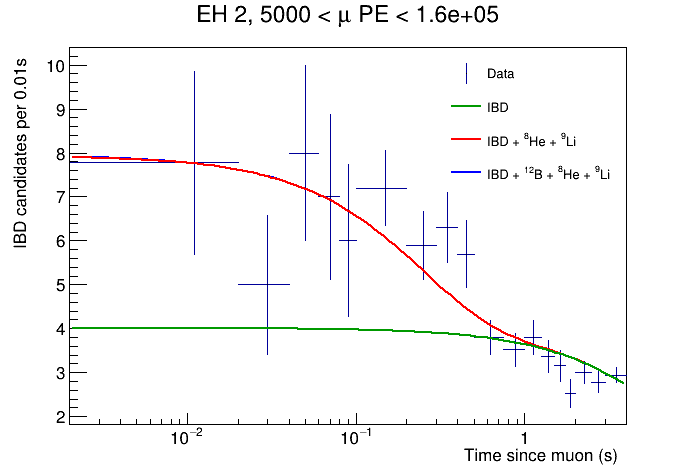
\includegraphics[width=0.5\linewidth]{Backgrounds/Li9/fits/EH2_range1_CV_logx.png} \\[0.5em]
  \begin{minipage}{0.5\textwidth}%
    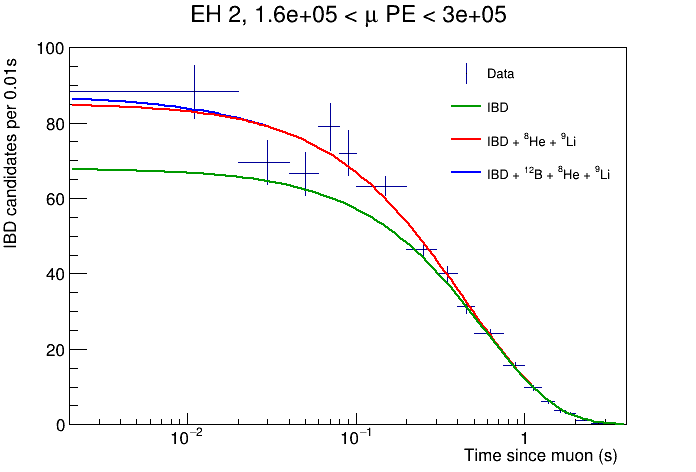
\includegraphics[width=\linewidth]{Backgrounds/Li9/fits/EH2_range2_CV_logx.png}%
  \end{minipage}%
  \begin{minipage}{0.5\textwidth}%
    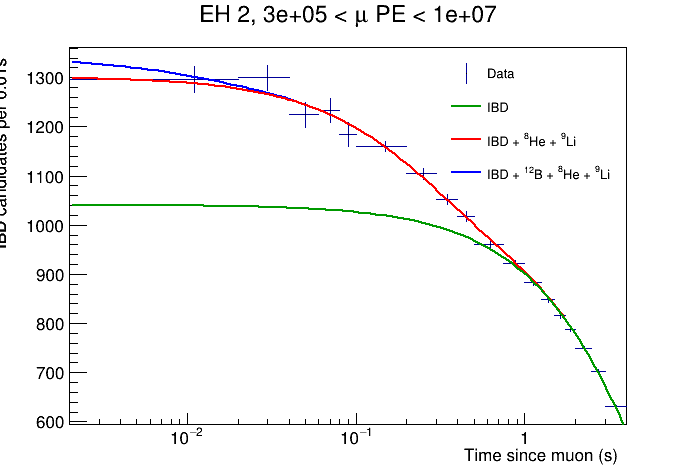
\includegraphics[width=\linewidth]{Backgrounds/Li9/fits/EH2_range3_CV_logx.png}%
  \end{minipage}%
  \caption{Time-to-last-muon fits for IBD-like events in EH2.}
  \label{fig:li9_fits_eh2}
\end{figure}

\begin{figure}[ht]
  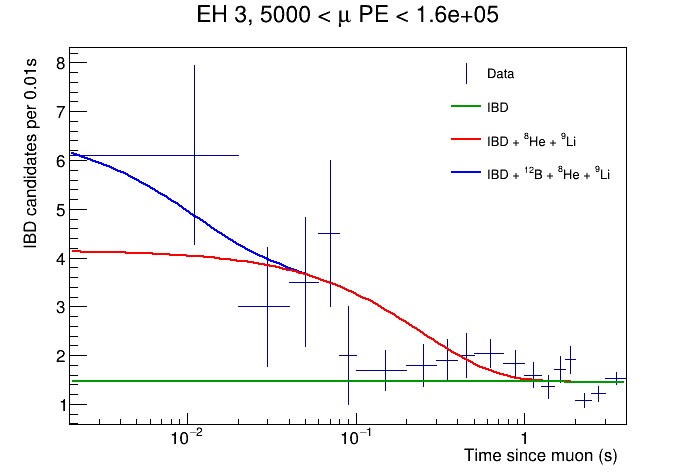
\includegraphics[width=0.5\linewidth]{Backgrounds/Li9/fits/EH3_range1_CV_logx.png} \\[0.5em]
  \begin{minipage}{0.5\textwidth}%
    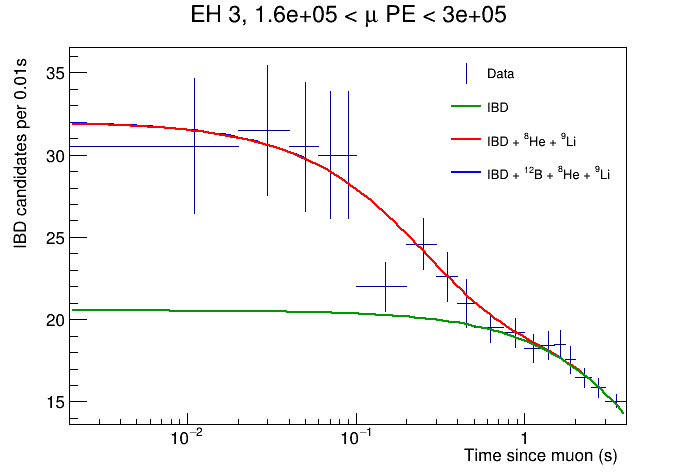
\includegraphics[width=\linewidth]{Backgrounds/Li9/fits/EH3_range2_CV_logx.png}%
  \end{minipage}%
  \begin{minipage}{0.5\textwidth}%
    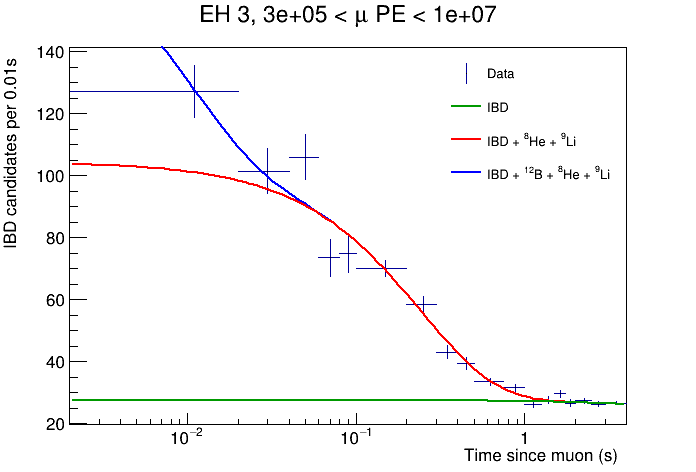
\includegraphics[width=\linewidth]{Backgrounds/Li9/fits/EH3_range3_CV_logx.png}%
  \end{minipage}%
  \caption{Time-to-last-muon fits for IBD-like events in EH3.}
  \label{fig:li9_fits_eh3}
\end{figure}

\begin{table}[h]
  \centering
  \begin{tabular}{lcc}
    \toprule
    Hall & PE range ($\times10^3$) & $N_{\mathrm{Bkg}}$ \\
    \midrule
    EH1  & Low (5-160)   & 164.0 $\pm$ 51.4 \\
         % & Mid (160-300) & 554.9 $\pm$ 0.2 \\
         & Mid (160-300) & 554.9 $\pm$ 200.5 \\
         & High (300-inf) & 6969.2 $\pm$ 675.4 \\
    \midrule
    EH2  & Low (5-160)   & 95.8 $\pm$ 27.4 \\
         % & Mid (160-300) & 301.7 $\pm$ 0.1 \\
         & Mid (160-300) & 301.7 $\pm$ 118.5 \\
         & High (300-inf) & 6282.7 $\pm$ 733.3 \\
    \midrule
    EH3  & Low (5-160)   & 66.8 $\pm$ 25.5 \\
         % & Mid (160-300) & 280.1 $\pm$ 67.5 \\
         & Mid (160-300) & 280.1 $\pm$ 89.4 \\
         & High (300-inf) & 1915.1 $\pm$ 182.4 \\
    \bottomrule
  \end{tabular}
  \caption{Measured number of $^9$Li+$^8$He events, as determined by the time-to-last-muon fit, for each hall and range of muon energies. Quoted errors are the statistical uncertainties reported by the fitter. No efficiency corrections have been applied.}
  \label{tab:bkgLi9Rates}
\end{table}
% NB: For mid-range, took relative errors from matt_li9_rates.txt (320k).

\subsection{Selection efficiencies and their uncertainties}
\label{sec:bkgLi9SelEffs}

\subsubsection{Prompt-energy cut}
\label{sec:bkgLi9PromptCutEff}

To determine the efficiences (and the corresponding uncertainties) of the prompt-energy cuts, we replicate the procedure developed in \cite{ChrisLi9}.\footnote{We deviate from \cite{ChrisLi9} in using a muon cut of 300,000~PE, rather than 400,000~PE, when selecting the $^9$Li-enriched sample used in the efficiency determination.} These efficiencies can simply be calculated by integrating the normalized $^9$Li spectrum (expressed in reconstructed energy) over the energies above each cut. The difficulty, however, lies in obtaining this spectrum. When subtracting the $^9$Li background from the spectrum of IBD candidates, we follow the tradition of using Ochoa's theoretical calculation of the spectrum, as described in \autoref{sec:bkgLi9Spectrum}. However, for the prompt-energy cut efficiencies, we extract the $^9$Li reconstructed spectrum directly from data.
% (TODO: Compare efficiencies from integrating Pedro's spectra.)
% We briefly describe his method here.

The spectrum extraction proceeds in two steps. First, a spectrum is obtained from a sample that is enriched in $^9$Li, and then a $^9$Li-deficient sample (consisting mainly of IBD ``background'') is acquired, rescaled, and subtracted from the $^9$Li-rich sample. This procedure produces a spectrum that contains very little contamination and can thereby give a reliable measurement of the prompt-energy cut efficiency.

To obtain the $^9$Li-rich sample, the $^9$Li candidates from all three halls were combined, and a subset was taken by selecting events that fell between 2 and 200~ms after a high-energy shower muon, defined here as a muon that produced more then 300,000 photoelectrons of visible energy. The time-to-last-muon fit of \autoref{eq:bkgLi9FullExpr} was then performed, giving the relative fraction of the sample comprised by \emph{shower-correlated} $^9$Li. The remaining, shower-uncorrelated, events consisted largely of non-$^9$Li ``background'' (predominantly true IBDs).

Within the shower-uncorrelated fraction, we expect the presence of some $^9$Li events produced by sub-300,000 p.e. muons, but this is a small contribution. As shown by the fit results in \autoref{tab:bkgLi9Rates}, some $f = 90\%$ of the total $^9$Li sample (before applying any shower-muon veto) is produced by showers of at least 300,000 photoelectrons. Meanwhile (as can be seen from visually inspecting the fits in Figures~\ref{fig:li9_fits_eh1}--\ref{fig:li9_fits_eh3}), in this muon energy range (and time window), the correlated events take up approximately $R = 1/3$ of the candidate sample. As such, the number of shower-uncorrelated $^9$Li events in this subsample, relative to the total number of uncorrelated events, is roughly
\begin{equation}
  \label{eq:bkgLi9SpecExtractErr}
  \begin{aligned}
    F &= \frac{(1 - f)R}{1 - R} = \frac{(1 - 0.9) \cdot 0.33}{1 - 0.33} \\
    &\approx 5\%
  \end{aligned}
\end{equation}
That is, the uncorrelated rate, as reported by the fit, describes a set that is about 95\% non-$^9$Li. Following \cite{ChrisLi9}, in what follows we assume that 95\% $\approx$ 100\%. It would be more correct to scale the non-$^9$Li ``background'' spectrum (described later) by $\sim$0.95 before subtracting it. In practice, we choose to simply assign an additional 5\% systematic uncertainty to account for this issue.
% We also ignore the effects of $^{12}$B, which amount to only a few percent, as seen from the plotted fits.

Given that around 2/3 of the events in this enriched sample are in fact non-$^9$Li ``background'' (mainly IBDs), it is imperative to obtain a clean background sample for subtraction. To do so, we use events from the $^9$Li selection which were preceded by at least 1.5~s of isolation from muons of greater than 200,000~pe. This cut excludes virtually all (99.8\%, based on the $^9$Li lifetime) $^9$Li events produced by $>$200,000~pe muons. The remaining $^9$Li events are a very small contribution: About 0.4\% of the (full) $^9$Li candidate sample consists of actual $^9$Li (according to the fits), and from \autoref{tab:bkgLi9Rates}, it can be seen that, at most, 15\% of these events are produced by muons of below 300,000~pe, and hence an even smaller percentage are produced by sub-200,000~pe muons. Conservatively taking 15\%, and multiplying it by 0.4\%, we derive an upper bound of 0.06\% on the level of $^9$Li contamination in the ``background'' sample. This is more than acceptable. Meanwhile, the overall rate of $^{12}$B events is less than 10\% of the $^9$Li rate (Figures~\ref{fig:li9_fits_eh1}--\ref{fig:li9_fits_eh3}), so they are even less of a concern.

Once the ``signal''\footnote{Signal + background, more precisely.} ($^9$Li) and ``background'' (IBD) samples were extracted, the background spectrum was scaled such that its integral equalled the number of shower-uncorrelated events in the signal sample (as reported by the time-to-last-muon fit), and then subtracted from the signal spectrum. The result was our final extracted $^9$Li spectrum (\autoref{fig:li9_spec}). The uncertainty in each bin, for both the signal and background spectra, were calculated based on Poisson statistics, and combined in quadrature to give the error bar on each bin of the spectrum. Finally, the efficiency of each prompt-energy cut was calculated by summing the counts of each accepted bin, and dividing this by the total count in all bins. The statistical uncertainty, meanwhile, was simply the result of adding the error on each bin in quadrature, and propagating the combined errors through the calculation of the ratio. As a cross-check, the calculation was performed separately for each hall, with the results found to be consistent with each other, validating the combination of all three halls in calculating a single efficiency.

Two potential sources of systematic uncertainty are considered in the calculation of the prompt-energy cut efficiency.\footnote{We directly use the results from \cite{ChrisLi9}, without repeating the procedure.} The first is the choice of time binning used. In \cite{ChrisLi9}, the efficiency analysis was repeated for the two alternative binnings described in \autoref{sec:bkgLi9Binning}, revealing a variation of less than 1\%. The second potential uncertainty arises from the choice of muon energy cut used in extracting the $^9$Li-deficient sample. When the cut was increased to 400,000~pe, the result was again a sub-1\% variation in the calculated efficiency \cite{ChrisLi9}. Based on these studies, we assign a total systematic uncertainty of 1\% (absolute) to the prompt cut efficiency.

The efficiencies and uncertainties for the three prompt-energy cuts are summarized in \autoref{tab:bkgLi9PromptCutEffs}. For each hall, the total uncertainty arising from the cut was determined from a weighted sum of the efficiencies that correspond to each muon PE range:
\begin{equation}
  \label{eq:bkgLi9PromptEffUnc}
  \sigma_p = \frac{w^{\mathrm{low}} \sigma_p^{\mathrm{low}} + w^{\mathrm{mid}} \sigma_p^{\mathrm{mid}} + w^{\mathrm{high}} \sigma_p^{\mathrm{high}}}{w^{\mathrm{low}} + w^{\mathrm{mid}} + w^{\mathrm{high}}},
\end{equation}
where $\sigma_p^{\mathrm{low}}$ is the uncertainty (statistical + systematic, in quadrature) of the efficiency of the prompt-energy cut used for the low muon PE range (and similarly for ``mid'' and ``high''). Meanwhile, the weights $w$ are proportional to the contribution of each range to the predicted daily rate (compare to \autoref{eq:bkgLi9DailyRate}):
\begin{equation}
  \label{eq:bkgLi9Weights}
  \begin{aligned}
    w^{\mathrm{low}} &= \frac{N^{\mathrm{low}}}{\epsilon_p^{\mathrm{low}}\epsilon_n} \\
    w^{\mathrm{mid}} &= \frac{N^{\mathrm{mid}}}{\epsilon_p^{\mathrm{mid}}} \\
    w^{\mathrm{high}} &= \left( \frac{f_{\mathrm{He}}}{e^{t_{\mathrm{sh}} / \tau_{\mathrm{He}}}} + \frac{1 - f_{\mathrm{He}}}{e^{t_{\mathrm{sh}} / \tau_{\mathrm{Li}}}} \right) \frac{N^{\mathrm{high}}}{\epsilon_p^{\mathrm{high}}}.
  \end{aligned}
\end{equation}
Here, $N^{\mathrm{low}}$ etc.\ are the values of $N_{\mathrm{bkg}}$ for the three PE ranges in \autoref{tab:bkgLi9Rates}, $\epsilon_p^{\mathrm{low}}$ etc.\ are the corresponding prompt efficiencies (Tables~\ref{tab:bkgLi9Cuts} and \ref{tab:bkgLi9PromptCutEffs}), $\epsilon_n$ is the neutron tagging efficiency (discussed in \autoref{sec:bkgLi9NeuTagEff}), $f_{\mathrm{He}}$ is the nominal $^8$He fraction of 5.5\%, $t_{\mathrm{sh}}$ is the shower veto time (0.4004~s), and $\tau_{\mathrm{Li}}$ ($\tau_{\mathrm{He}}$) is the $^9$Li ($^8$He) lifetime. The results are shown in
% \autoref{tab:bkgLi9NetPromptCutUnc}.
\autoref{tab:bkgLi9UncSumm}.

\begin{table}[h]
  \centering
  \begin{tabular}{lc}
    \toprule
    Prompt energy cut & Efficiency \\
    \midrule
    3.5 MeV & $78.3\% \pm 5.4\%\, \text{(stat.)} \pm 1\%\, \text{(syst.)}$\\
    6 MeV & $43.0\% \pm 2.9\%\, \text{(stat.)} \pm 1\%\, \text{(syst.)}$\\
    8 MeV & $16.8\% \pm 1.4\%\, \text{(stat.)} \pm 1\%\, \text{(syst.)}$\\
    \bottomrule
  \end{tabular}
  \caption{Prompt-energy cut efficiencies for the $^9$Li selection.}
  \label{tab:bkgLi9PromptCutEffs}
\end{table}

% \begin{table}[ht]
%   \begin{tabular}{lc}
%     \toprule
%     Hall & $\sigma_p$ \\
%     \midrule
%     EH1 & 2.8\% \\
%     EH2 & 3.3\% \\
%     EH3 & 4.0\% \\
%     \bottomrule
%   \end{tabular}
%   \caption{Uncertainty of the $^9$Li rate arising from the efficiency of the prompt energy cut, per \autoref{eq:bkgLi9PromptEffUnc}.}
%   \label{tab:bkgLi9NetPromptCutUnc}
% \end{table}

\subsubsection{Neutron tagging}
\label{sec:bkgLi9NeuTagEff}

Historically, the largest contribution to the overall $^9$Li rate uncertainty has come from the neutron tagging efficiency. In previous analyses, the prompt-energy cut was 3.5~MeV, for which the IBD ``background'' was so large as to require neutron tagging for all muons below 300,000~pe. Given that some 60-70\% of the total $^9$Li rate \footnote{In the oscillation analysis, i.e., with the shower-muon veto.} comes from muons below 300,000~pe, this uncertainty applied to that entire subsample. Making matters worse, this uncertainty is quite large, as the efficiency can only be directly measured for higher-energy muons (where neutron tagging is not necessary in order to obtain a valid time-to-last-muon fit). The efficiency must thus be extrapolated (with considerable uncertainty) for lower-energy muons. Owing to our use of a stricter prompt-energy cut (of 8~MeV and 6~MeV in the near and far halls, respectively) for muons below 300,000~pe, the neutron tagging requirement has been eliminated in the range of 160,000--300,000~pe, significantly reducing the total uncertainty from neutron tagging. However, for 5,000--160,000~pe (which contributes 12--16\% of the final $^9$Li rates), where neutron tagging remains unavoidable, the extrapolated efficiency must still be used.

In \cite{WeiLi9}, the efficiency was found to range from about 60 to 100\% within the energy ranges where it could be measured directly. As such, an uncertainty of 45\% was assigned in \cite{ChrisLi9} to the efficiency, with a nominal value of unity. This latter choice can be post-hoc justified by the results in \cite{MaWuLi9}, where an efficiency of 93.9\% was found for 160,000 to 400,000~pe in EH1; nevertheless, values closer to 70\% were found in the other two halls, and the efficiency is expected to decrease for lower muon energies. % Based on these results, we deviate from Marshall in assuming an efficiency of 60\%.
% (YYY need to update numbers; previously used 100\%.)
Although a lower efficiency might be more accurate, we use unity for the sake of consistency with \cite{ChrisLi9}. In any case,
% the efficiency is only relevant for the $^9$Li nuclei produced by sub-160,000 muons, which contribute merely 2--10\% of the final $^9$Li rate in our IBD candidate sample,\footnote{See \autoref{tab:bkgLi9Rates}. Note that the shower muon veto in the IBD selection results in a reduction of $\sim$80\% for the events in the ``High'' PE range.} The value chosen for this efficiency thus has only marginal impact on the calculated rate. Furthermore,
the 45\% uncertainty encompasses the range of values observed in \cite{MaWuLi9}.

% Owing to our use of much stricter prompt-energy cut for muons below 300,000~pe (8 MeV and 6 MeV in the near and far halls, respectively), neutron tagging is no longer necessary in the muon energy range of 160,000 to 300,000~pe. This range contributes to about 60\% of the total $^9$Li background, out of the 80\% that previously required neutron reduction. The more stringent prompt-energy cut thereby reduces the total uncertainty by some 25\% in the near halls. In the far halls, where the mean muon energy is significantly higher (and thus the muons that require neutron tagging contribute a relatively minor proportion of the total $^9$Li rate), the stricter prompt-energy cut has a relatively minor effect.

The uncertainty on the final $^9$Li rate resulting from the neutron tagging efficiency, for each hall, is equal to 45\% scaled by the proportion of $^9$Li events that come from muons of 5,000--160,000~pe (the ``low'' range):
\begin{equation}
  \sigma_n = \frac{w^{\mathrm{low}}}{w^{\mathrm{low}} + w^{\mathrm{mid}} + w^{\mathrm{high}}} \cdot 0.45,
\end{equation}
where the weights $w$ were given previously in \autoref{eq:bkgLi9Weights}. The values for each hall are shown in \autoref{tab:bkgLi9UncSumm}.

% 7.2%, 6.4%, 5.3%

\subsection{Other systematics}
\label{sec:bkgLi9FitSyst}

\subsubsection{Variation of neutron tagging cutoff}
\label{sec:bkgLi9NeuTagCutoff}

In our $^9$Li fits, neutron tagging is applied for muons below 160,000~pe. To study the effects of varying this dividing line, the analysis was repeated in \cite{ChrisLi9} for various values, ranging from 150,000 to 180,000~pe. The resulting variation in the final estimated rate of $^9$Li was found to be of order 10\%. We assign this value verbatim as an additional systematic uncertainty on the final rate.

\subsubsection{Binning}
\label{sec:bkgLi9Binning}

To study the effect of varying the time binning used in the fit,\footnote{As described above, 25 variable-width bins from 0.002 to 10 seconds, with 20~ms bins below 100~ms} two alternative binnings were tested in \cite{ChrisLi9}. The first was finer, with 40 total bins and 10-ms bins below 100~ms. The second was coarser, with 20 total bins and 50-ms bins below 100~ms. These alternative binnings produced less than a 5\% shift in the final result. Accordingly, we assign a 5\% systematic uncertainty to account for the effect of binning.

\subsubsection{$^{12}$B and $^8$He components}
\label{sec:bkgLi9B12unc}

Our fits assume a 5.5\% nominal $^8$He fraction and include a component correspond to $^{12}$B.
% As shown in \autoref{fig:bkgLi9Linreg}, the (XXX)
To characterize the sensitivity of the analysis to these choices, the fit was repeated after disabling the $^{12}$B component and after varying the $^8$He fraction from 0 to 15\%. These variations shifted the final rate by some 10\%, which we assign as an additional systematic uncertainty.

The $^8$He fraction, in addition to affecting the result of the fit, also affects the conversion into the final daily rate (described in the next section). This is because a correction factor must be applied to account for the shower-muon veto used in the IBD selection. The efficiency of this veto is a function of the isotope livetime, which of course varies between $^9$Li and $^8$He.\footnote{This systematic uncertainty in this shower-muon veto survival probability, resulting from the uncertainty in the $^8$He fraction, was not considered in \cite{ChrisLi9}.}

We consider three cases: 0\% $^8$He, 5.5\% $^8$He (the nominal fraction), and 15\% $^8$He. For the nominal shower-muon veto of $\sim$0.4~s, the three efficiencies are, respectively,
\begin{align*}
  \exp(-0.4/0.257) &= 0.211 \\
  0.945 \times \exp(-0.4/0.257) + 0.055 \times \exp(-0.4/0.172) &= 0.205 \\
  0.85 \times \exp(-0.4/0.257) + 0.15 \times \exp(-0.4/0.172) &= 0.194.
\end{align*}
Taking the spread of these three values (0.017), and dividing by the mean (0.203), we find a relative spread of 0.084, corresponding to an uncertainty of roughly 4\% in the final rate for $^9$Li events produced by muons above 300,000~pe (our nominal shower-muon cut in the oscillation IBD selection). Given that these high-energy muons produce some 30-40\% of the final $^9$Li events in the sample (after the shower-muon veto), we conservatively assign 2\% (half of 4\%) as an additional systematic uncertainty on the total $^9$Li rate. % In \autoref{fig:bkgLi9Linreg}, we plot the dependence of the $^9$Li measurement on the assumed $^8$He fraction (and on whether $^{12}$B is included in the fit.)

\subsection{Summary of uncertainties}
\label{sec:bkgLi9UncSumm}

The uncertainty budget of the $^9$Li rate is shown in \autoref{tab:bkgLi9UncSumm}. The various systematic uncertainties were discussed in the preceding sections. To obtain the (relative) statistical uncertainties, first, the absolute statistical uncertainties were calculated by inserting the uncertainties in the various $N_{\mathrm{Bkg}}$ (from \autoref{tab:bkgLi9Rates}) into \autoref{eq:bkgLi9DailyRate}, and then these were divided by the rates (calculated by inserting the $N_{\mathrm{Bkg}}$ values themselves into \autoref{eq:bkgLi9DailyRate}, as described in \autoref{sec:bkgLi9DailyRateCalc}). The individual uncertainties were added in quadrature to obtain each hall's total uncertainty.

\begin{table}[ht]
  \begin{tabular}{lccc}
    \toprule
    Uncertainty & EH1 (\%)& EH2 (\%) & EH3 (\%) \\
    \midrule
    Statistical & 27.5 & 26.5 & 24.1 \\
    Spectrum extraction (see \autoref{eq:bkgLi9SpecExtractErr}) & 5.0 & 5.0 & 5.0 \\
    Prompt-energy cut efficiency & 2.8 & 3.3 & 4.0 \\
    Neutron tagging efficiency & 7.2 & 6.4 & 5.3 \\
    Neutron tagging cutoff & 10.0 & 10.0 & 10.0 \\
    Binning & 5.0 & 5.0 & 5.0 \\
    $^{12}$B component and $^8$He fraction (fitting) & 10.0 & 10.0 & 10.0  \\
    $^8$He component (veto survival probability) & 2.0 & 2.0 & 2.0 \\
    \midrule
    Total & 32.7 & 31.7 & 29.6 \\
    \bottomrule
  \end{tabular}
  \caption{Uncertainty budget for the $^9$Li/$^8$He rate.}
  \label{tab:bkgLi9UncSumm}
\end{table}

\subsection{Calculation of daily rates}
\label{sec:bkgLi9DailyRateCalc}

Based on the results of fitting the three muon energy ranges, the final daily $^9$Li rate per AD in each hall is calculated as
\begin{equation}
  \label{eq:bkgLi9DailyRate}
%   \begin{aligned}
%   \frac{1}{\epsilon_\mu \epsilon_m T N^{\mathrm{eff}}_{\mathrm{det}}}
%   \left\{ \phantom{(1-f_{\mathrm{He}})\left[ \frac{N^{\mathrm{low}}}{\epsilon^{\mathrm{low}}_p \epsilon_n} 
%           + \frac{N^{\mathrm{mid}}}{\epsilon_p^{\mathrm{mid}}}
%           % + \frac{N^{\mathrm{low}}}{\epsilon_p^{\mathrm{low}} \exp(-t_{\mathrm{sh}} / \tau_{\mathrm{Li}})}
%           + \frac{N^{\mathrm{high}}}{\epsilon_p^{\mathrm{high}} e^{t_{\mathrm{sh}} / \tau_{\mathrm{Li}}}}\right]}
%         \right.
      % & (1-f_{\mathrm{He}})\left[ \frac{N^{\mathrm{low}}}{\epsilon^{\mathrm{low}}_p \epsilon_n} 
      %   + \frac{N^{\mathrm{mid}}}{\epsilon_p^{\mathrm{mid}}}
      %   % + \frac{N^{\mathrm{low}}}{\epsilon_p^{\mathrm{low}} \exp(-t_{\mathrm{sh}} / \tau_{\mathrm{Li}})}
      %   + \frac{N^{\mathrm{high}}}{\epsilon_p^{\mathrm{high}} e^{t_{\mathrm{sh}} / \tau_{\mathrm{Li}}}}
%       \right] \\
%       & \left.
%         f_{\mathrm{He}}\left[ \frac{N^{\mathrm{low}}}{\epsilon^{\mathrm{low}}_p \epsilon_n} 
%         + \frac{N^{\mathrm{mid}}}{\epsilon_p^{\mathrm{mid}}}
%         % + \frac{N^{\mathrm{low}}}{\epsilon_p^{\mathrm{low}} \exp(-t_{\mathrm{sh}} / \tau_{\mathrm{He}})}
%         + \frac{N^{\mathrm{high}}}{\epsilon_p^{\mathrm{high}} e^{t_{\mathrm{sh}} / \tau_{\mathrm{He}}}}
%       \right] \right\},
% \end{aligned}
  \frac{1}{\epsilon_\mu \epsilon_m T N^{\mathrm{eff}}_{\mathrm{det}}}
  \left[  \frac{N^{\mathrm{low}}}{\epsilon^{\mathrm{low}}_p \epsilon_n} 
    + \frac{N^{\mathrm{mid}}}{\epsilon_p^{\mathrm{mid}}}
    + \left( \frac{f_{\mathrm{He}}}{e^{t_{\mathrm{sh}} / \tau_{\mathrm{He}}}} + \frac{1 - f_{\mathrm{He}}}{e^{t_{\mathrm{sh}} / \tau_{\mathrm{Li}}}} \right) \frac{N^{\mathrm{high}}}{\epsilon_p^{\mathrm{high}}}
  \right]
\end{equation}
where $\epsilon_\mu$ is the efficiency of the muon veto (without the shower-muon veto), $e_m$ is the multiplicity cut efficiency, $T$ is the total livetime, $N^{\mathrm{eff}}_{\mathrm{det}}$ is the livetime-weighted number of detectors, $N^{\mathrm{low/mid/high}}$ are the raw rates from the fits (as listed in \autoref{tab:bkgLi9Rates}), $\epsilon_n = 1$ is the neutron-tagging efficiency, $\epsilon_p$ are the prompt-energy cut efficiencies (~\autoref{tab:bkgLi9PromptCutEffs}), $f_{\mathrm{He}} = 5.5\%$ is the nominal $^8$He fraction, $\tau_{\mathrm{Li}}$ ($\tau_{\mathrm{He}}$) is the $^9$Li ($^8$He) lifetime, and $t_{\mathrm{sh}}$ is the shower-muon veto time of 0.4004~s. As mentioned earlier, the muon-veto efficiencies are calculated using the toy MC described in \autoref{sec:cutVaryMuVetoEff}, and the multiplicity cut efficiencies (which are relatively stable) are taken from the IBD selection.\footnote{The multiplicity efficiencies are 97-98\%; the 2-3\% inefficiency is negligible in comparison to the overall $^9$Li uncertainty, so we need not dwell on it any further.} The relative uncertainties, as calculated in \autoref{sec:bkgLi9UncSumm}, were scaled by the rates to give the absolute uncertainties quoted in the table.

\begin{table}[h]
  \begin{tabular}{lccccc}
    \toprule
    Hall & $\epsilon_\mu$ & $\epsilon_m$ & $T$ (days) & $N_{\mathrm{det}}^{\mathrm{eff}}$ & Events/AD/day \\
    \midrule
    EH1 & 0.8711 & 0.9772 & 1737 & 1.8888 & 2.18 $\pm$ 0.71 \\
    EH2 & 0.9015 & 0.9782 & 1729 & 1.8925 & 1.39 $\pm$ 0.44 \\
    EH3 & 0.9883 & 0.9829 & 1737 & 3.8921 & 0.199 $\pm$ 0.059 \\
    \bottomrule
  \end{tabular}
  \caption{Final estimates of the daily $^9$Li rate (per AD) in each hall, according to \autoref{eq:bkgLi9DailyRate}. Note that, since the efficiencies of the muon veto and multiplicity cut (in the $^9$Li+$^8$He selection) were divided out in \autoref{eq:bkgLi9DailyRate}, we must multiply these rates by the corresponding efficiencies of our IBD selection in order to obtain the predicted number of $^9$Li+$^8$He events in our raw IBD sample.}
  \label{tab:bkgLi9DailyRates}
\end{table}

\subsection{Linear regression}
\label{sec:bkgLi9LinReg}

When we experiment with modifying the charge threshold and veto time of the shower muon veto, as described in \autoref{chap:cutVary}, the $^9$Li rate must be recalculated using \autoref{eq:bkgLi9DailyRate} for each case. Although the modified value of $\tau$ can simply be inserted into the equation, there is also an implicit dependence on the charge threshold, which determines the division of muons between the mid- and high-energy bins. Although it would be possible to repeat the $^9$Li selection for each value of the threshold, this would be a rigid and time-consuming approach. Instead, we perform the selection at 44 evenly-spaced values of the mid/high dividing line, ranging from $1.7\times10^5$ to $6.0\times10^5$ PE\@. When our threshold lies in between these grid points, we must interpolate.

Our initial approach was to simply perform a linear interpolation between the two points on each side of the threshold. This would be done once for the mid-energy bin, and again for the high-energy bin. However, the results of the $^9$Li selection/fit demonstrate a fair amount of random jitter between adjacent values of the mid/high threshold, as shown in Figures~\ref{fig:li9_linreg_eh1}--\ref{fig:li9_linreg_eh3}. Although this variation is well below the systematic uncertainty on the $^9$Li rate, it does introduce artificial structure to the results of the shower-muon veto variation. Fortunately, the $^9$Li rates show a fairly linear dependence on the threshold, as shown in the same plots. Therefore, our approach is to calculate the $^9$Li rate using \autoref{eq:bkgLi9DailyRate} at each of the 44 grid points for the charge threshold (using the same modified veto time in each case), fit the results to a line, and then evaluate this line at the desired value for the threshold.
% As is shown, we also vary the assumptions on the $^8$He fraction and the presence of $^{12}$B; all four sets of results are used in the linear regression.
This procedure produces the $^9$Li rate that is used in the oscillation fit for arbitrary shower-muon veto parameters in \autoref{chap:cutVary}.

\begin{figure}[ht]
  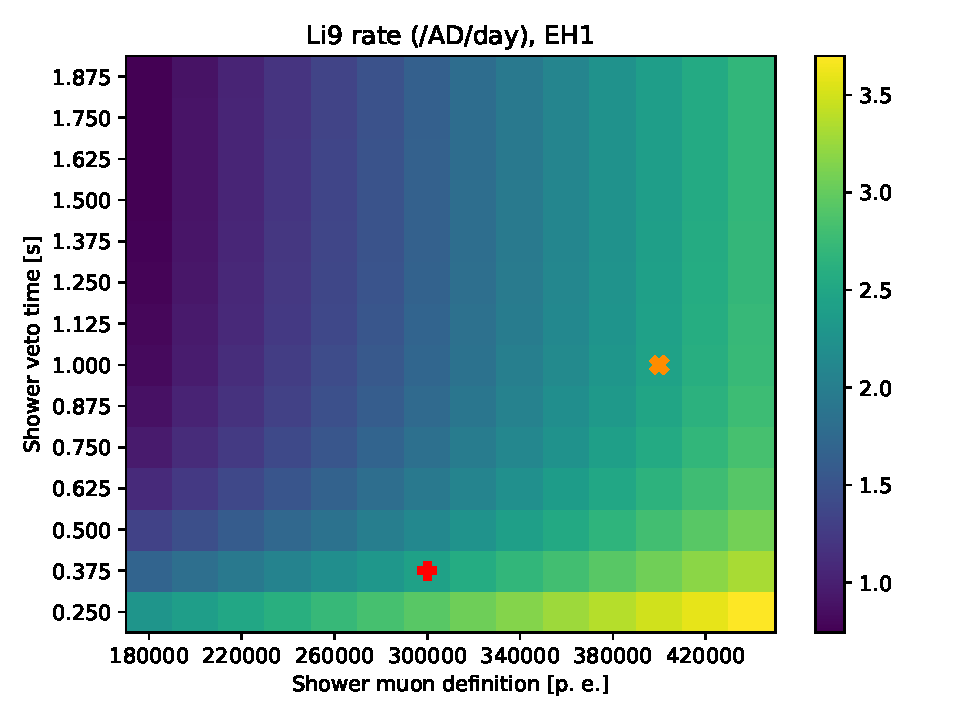
\includegraphics[width=0.7\textwidth]{Backgrounds/Li9/linreg/li9_linreg_eh1.pdf}
  \caption{Dependence of the measured $^9$Li rate (for the nominal shower-muon veto time of 400.4~ms) on the shower-muon threshold in EH1. The line-of-best-fit is used in determining the $^9$Li rate for arbitrary shower-muon tresholds in \autoref{chap:cutVary}.}
  \label{fig:li9_linreg_eh1}
\end{figure}

\begin{figure}[ht]
  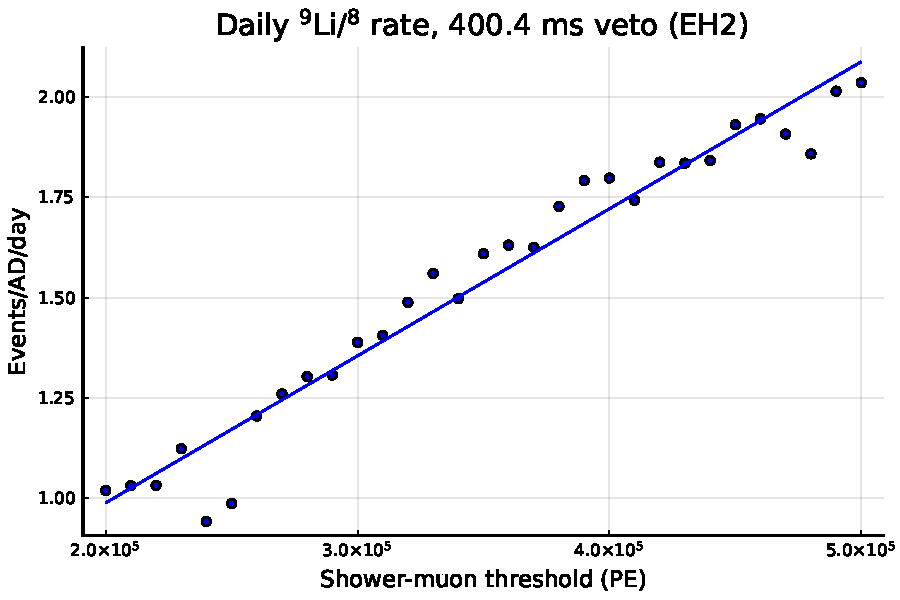
\includegraphics[width=0.7\textwidth]{Backgrounds/Li9/linreg/li9_linreg_eh2.pdf}
  \caption{Dependence of the measured $^9$Li rate (for the nominal shower-muon veto time of 400.4~ms) on the shower-muon threshold in EH2. The line-of-best-fit is used in determining the $^9$Li rate for arbitrary shower-muon tresholds in \autoref{chap:cutVary}.}
  \label{fig:li9_linreg_eh2}
\end{figure}

\begin{figure}[ht]
  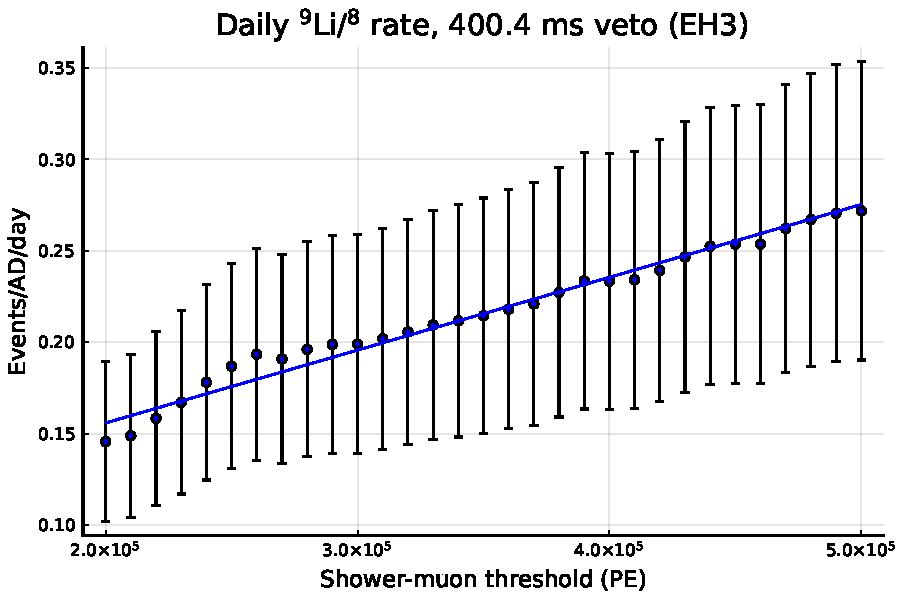
\includegraphics[width=0.7\textwidth]{Backgrounds/Li9/linreg/li9_linreg_eh3.pdf}
  \caption{Dependence of the measured $^9$Li rate (for the nominal shower-muon veto time of 400.4~ms) on the shower-muon threshold in EH3. The line-of-best-fit is used in determining the $^9$Li rate for arbitrary shower-muon tresholds in \autoref{chap:cutVary}.}
  \label{fig:li9_linreg_eh3}
\end{figure}


\begin{comment}
- forming and fitting the histogram %
- - Detail the cuts we use for different muon energy ranges (prompt energy, neutron tag)
- Prompt cut efficiency
- - Extraction of spectrum. Subtraction of IBD spectrum.
- - Uncertainty
- - - Statistical - binomial confidence interval accounting for error bars on subtracted spectrum => 1-2\% (See if can find how Chris did it in code... sounds tricky)
- - - Systematic - Variations in time binning, muon PE cut in background sample => 1\%
- Neutron tag efficiency
- - Uncertainty - 45\% according to doc-10920
- - Nominal value of... 80\%? 60\%?
- Uncertainty from fit
- - Neutron tagging cutoff - 1.5e5 to 1.8e5 => 10\% (NOT IN CHRIS'S TABLE)
- - Binning => <5\% (NOT IN CHRIS'S TABLE) (MENTIONED AT END)
- - B12 => 8\%
- - He8 => 4\%
- Uncertainty of shower veto correction (He8 fraction)
- - Vary He8 fraction from 0 to 15\%
- Conversion from fit result to daily rate
- - Efficiencies of Li9 selection (ntag, pcut)
- - IBD selection efficiencies (veto, mult)
- - Shower veto correction
- - Propagation of uncertainties
\end{comment}

\subsection{Spectrum}
\label{sec:bkgLi9Spectrum}

The \LiHe\ spectrum can be either extracted from data or predicted from nuclear tables. Both methods give consistent results (\autoref{fig:li9_spec}). The extracted spectrum (used for determining the efficiency of the prompt-energy cut in the $^9$Li selection) was described in \autoref{sec:bkgLi9PromptCutEff}. Largely for historical reasons, our background subtraction does not employ the extracted spectrum, instead using the predicted one. Here we briefly describe this prediction \cite{pedroLi9Spec1,pedroLi9Spec2}.

\begin{figure}[h]
  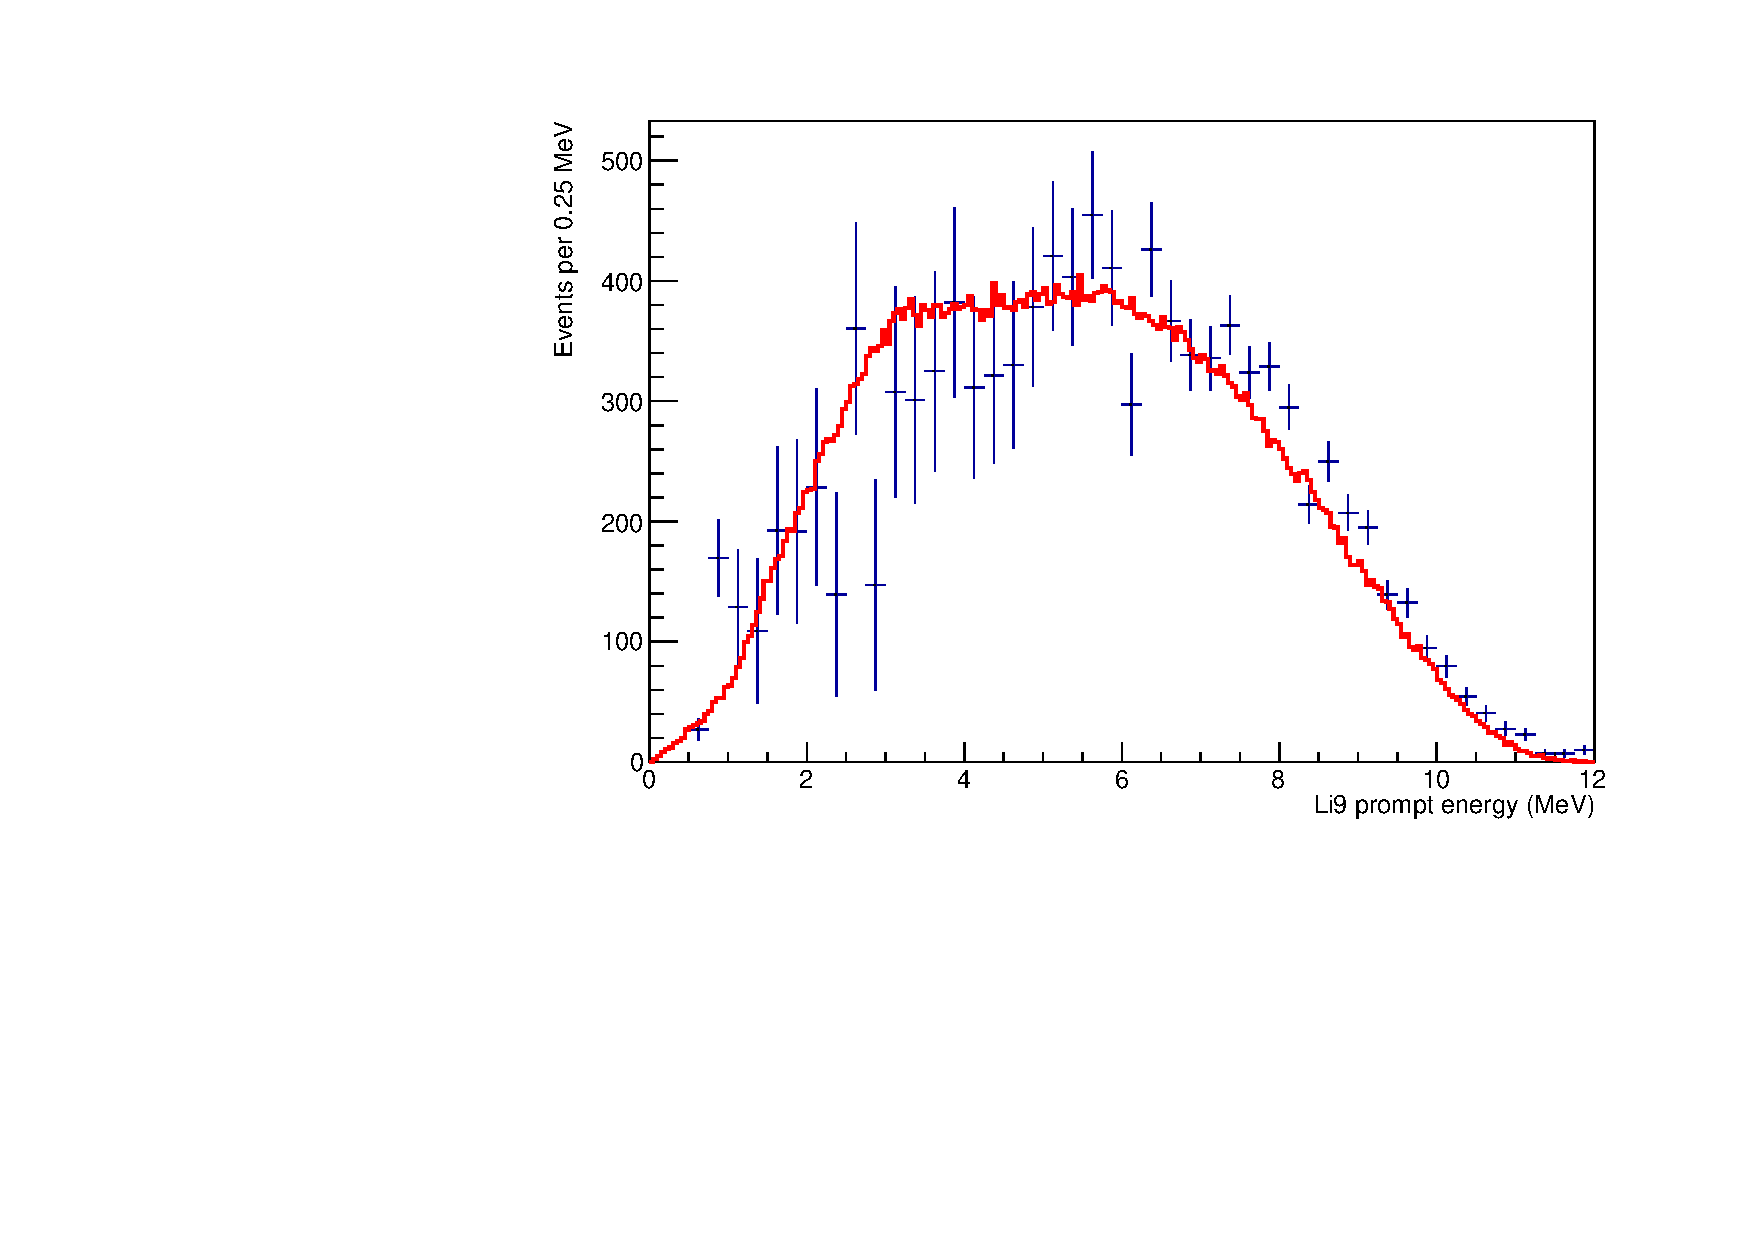
\includegraphics[width=0.5\textwidth]{Backgrounds/Li9/li9_spec_mine.pdf}
  \caption{Comparison of our extracted $^9$Li spectrum (blue points) with the predicted spectrum from \cite{pedroLi9Spec1,pedroLi9Spec2} (red line).}
  \label{fig:li9_spec}
\end{figure}

\begin{comment}
An extraction of the spectrum from Daya Bay data was performed by Marshall in [YYY]. The approach takes advantage of the fact that \LiHe\ are essentially the only IBD-like events that are correlated with muons on the 100~ms timescale. A \LiHe-enriched sample was obtained by taking IBD-like events within 2---200~ms of a ``shower'' muon, here defined as one producing at least $2\times10^5$ photoelectrons. This sample contained various muon-uncorrelated ``backgrounds'', such as true IBDs and accidentals. In order to remove this contamination, a \LiHe-depleted sample was obtained by looking for IBD candidates with no preceding shower muons within 1.5~s. Before subtracting the two spectra, an appropriate normalization for the depleted sample had to be determined. This was done by performing the time-to-last-muon fit for the enriched sample, which indicated the number of true \LiHe\ events in the sample, in turn implying the number of non-\LiHe\ events. The depleted sample was thus normalized to this latter count, and the subtraction was performed, giving the results shown in Fig.~YYY.
\end{comment}

For the prediction, three types of reference tables were consulted: nuclear structure, branching ratios, and measured spectra (of neutrons, alpha particles, and gamma-rays). Nuclear levels and decay schemes are shown in \Autoref{fig:li9_levels,fig:he8_levels}. Given the number of decay pathways involved, a purely analytic approach was infeasible (at least for $^9$Li), so a toy Monte Carlo was used to produce random decay events. The discussion here uses the example of $^9$Li, but $^8$He was essentially treated the same way. The initial $\beta$ decay (into any of four $^9\mathrm{Be}^*$ states) was simulated using the Fermi theory \cite{Fermi1934TentativoDU} and the published energy levels and branching fractions. For the decays that produce a $2\alpha+n$ final state (i.e. the only decays of interest to us), $^9\mathrm{Be}^*$ disintegrates via two consecutive two-body decays (via either $^8$Be or $^5$He). The angular distribution is assumed to be uniform. The disintegration was treated using basic kinematics, with the width of each state (\autoref{tab:bkgLi9Widths}) modeled with a Breit-Wigner function. The result was a collection of simulated events, each one recording the true energies of the electron, the neutron, and the two alphas (or, in the case of $^8$He, the electron, the neutron, and the gamma-ray).

\begin{figure}[h]
  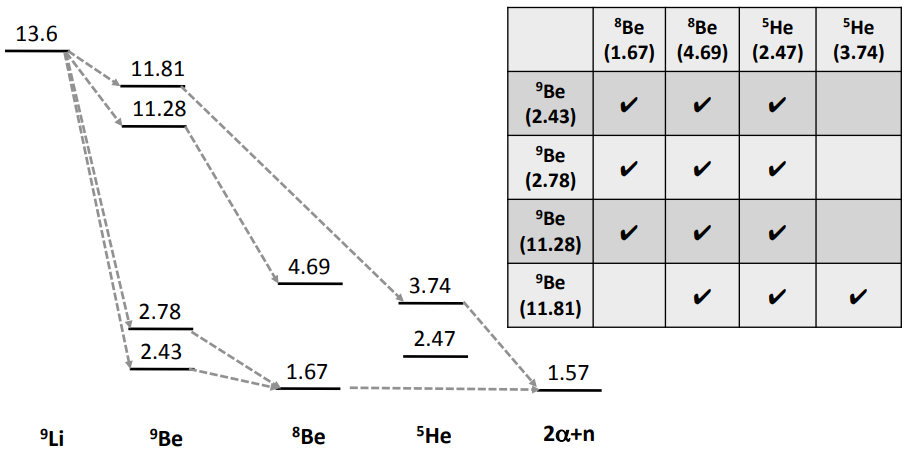
\includegraphics[scale=0.5]{Backgrounds/li9_levels.png}
  \caption{The decay of $^9$Li. Not all decays are shown with arrows. Energy levels are in MeV, relative to the ground state of $^9$Be. From \cite{pedroLi9Spec2}.}
  \label{fig:li9_levels}
\end{figure}

\begin{figure}[h]
  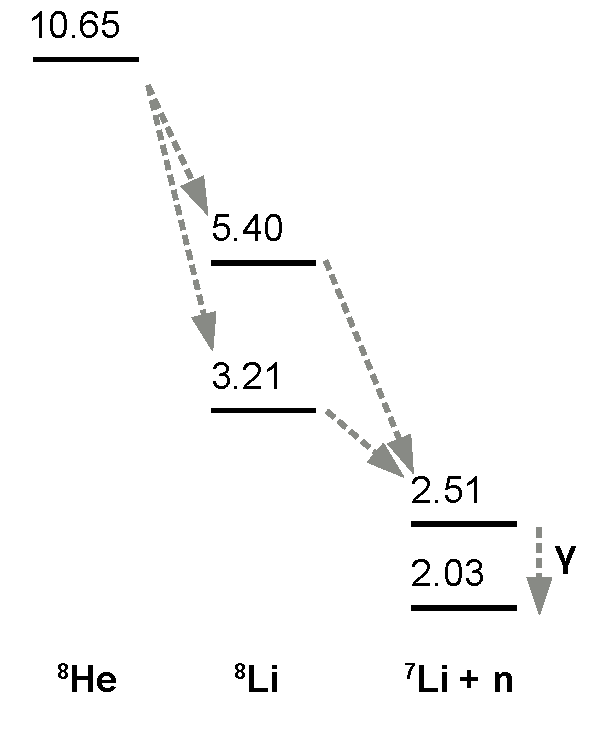
\includegraphics[scale=0.5]{Backgrounds/he8_levels.pdf}
  \caption{The decay of $^8$He. Energy levels are in MeV, relative to the ground state of $^8$Li.}
  \label{fig:he8_levels}
\end{figure}

\begin{table}[ht]
  \begin{tabular}{llcc}
    \toprule
    Parent & Daughter & Level (MeV) & Width (MeV) \\
    \midrule
    $^9$Li & $^9$Be & 11.81 & 0.400 \\
           & & 11.28 & 0.575 \\
           & & 2.78 & 0.110 \\
           & & 2.43 & $0.780 \times 10^{-3}$ \\
           & $^8$Be & 4.69 & $5.57 \times 10^{-6}$ \\
           & & 1.67 & 1.51 \\
           & $^5$He & 3.74 & 5.57 \\
           & & 1.67 & 0.648 \\
    \midrule
    $^8$He & $^8$Li & 5.40 & 0.650 \\
           & & 3.21 & 1.00 \\
           & $^7$Li & 2.51 & $9.02\times10^{-9}$ \\
           & & 2.03 & Stable \\
    \bottomrule
  \end{tabular}
  \caption{Widths of the nuclear excited states relevant for the prediction of the $^9$Li and $^8$He spectra \cite{ENDF}. For the daughters of $^9$Li ($^8$He), energy levels are expressed relative to the ground state of $^9$Be ($^8$Li).}
  \label{tab:bkgLi9Widths}
\end{table}

In order to benchmark this simulation, its output was compared against published measurements of \LiHe\ spectra of neutrons, alpha particles, and gamma-rays. Based on this comparison, one particularly broad level of $^8$He had to be augmented with a Gaussian density of states. Since the published branching ratios were relatively imprecise, they were hand-tuned (within limits) in the simulation so as to achieve satisfactory agreement with the published spectra.

Finally, to obtain the predicted spectrum in terms of prompt energy (i.e. reconstructed energy), the simulated events were passed through a model of the detector nonlinearity. Given that the \LiHe\ spectrum prediction was performed in 2013, it is based on an older nonlinearity model than the one discussed in \autoref{sec:fitToyDetResponse}.\footnote{The differences between models are not significant enough to warrant concern, especially in light of the uncertainty we assign to the \LiHe\ spectrum, as discussed in \cite{berkeley_toymc}.} Crucially, this model includes nonlinearity curves for the alpha particle and neutron, whose kinetic energies were also considered when determining the prompt energy for each event \cite{bcwNonlin}. The resulting prompt-energy spectra could then be combined according to the best estimate of the relative proportions of $^9$Li and $^8$He. For the sake of this analysis, a nominal 5.5\% fraction of $^8$He was used.\footnote{The measured spectrum and the rate fit both give results that are consistent with zero $^8$He, while rough predictions indicate that the $^8$He proportion should not exceed 20\%. (See the discussion of KamLAND on p.~\pageref{par:kamland_he8}.) Meanwhile, the predicted spectrum does not change very significantly when the fraction is varied from 0 to 15\%, in comparison to the other sources of uncertainty (neutron and alpha quenching). Hence, 5.5\%, an ``inherited'' feature of this analysis, is as good a guess as any.} \autoref{sec:fitToyBackgrounds} discusses the uncertainty assigned to the \LiHe\ spectrum.

\section{Cosmogenic fast neutrons}
\label{sec:bkgFastnOverview}

XXX see \autoref{sec:bkgFastn}.


\section{AmC source}
\label{sec:bkgAmCOverview}

XXX see \autoref{sec:bkgAmC}.


\section{$\CanO$}
\label{sec:bkgCanOOverview}

XXX see \autoref{sec:bkgCanO}.

\end{document}
